\documentclass[sigconf]{acmart}

\usepackage{float}
\usepackage{textgreek}

%encoding
%--------------------------------------
\usepackage[T1]{fontenc}
\usepackage[utf8]{inputenc}
%--------------------------------------

%Portuguese-specific commands
%--------------------------------------
\usepackage[brazilian]{babel}
%--------------------------------------

%Hyphenation rules
%--------------------------------------
\usepackage{hyphenat}
\hyphenation{mate-mática recu-perar}
%--------------------------------------

%Add codes and colors
%--------------------------------------
\usepackage{listings}
\usepackage{xcolor}
%--------------------------------------

%New colors defined below
\definecolor{codegreen}{rgb}{0,0.6,0}
\definecolor{codegray}{rgb}{0.5,0.5,0.5}
\definecolor{codepurple}{rgb}{0.58,0,0.82}
\definecolor{backcolour}{rgb}{0.95,0.95,0.92}

%Code listing style named "mystyle"
\lstdefinestyle{mystyle}{
  backgroundcolor=\color{backcolour},   commentstyle=\color{codegreen},
  keywordstyle=\color{magenta},
  numberstyle=\tiny\color{codegray},
  stringstyle=\color{codepurple},
  basicstyle=\ttfamily\footnotesize,
  breakatwhitespace=false,         
  breaklines=true,                 
  captionpos=b,                    
  keepspaces=true,                 
  numbers=left,                    
  numbersep=5pt,                  
  showspaces=false,                
  showstringspaces=false,
  showtabs=false,                  
  tabsize=2
}

%"mystyle" code listing set
\lstset{style=mystyle}

\AtBeginDocument{%
  \providecommand\BibTeX{{%
    \normalfont B\kern-0.5em{\scshape i\kern-0.25em b}\kern-0.8em\TeX}}}

\acmConference[Controle de Versão 2020.2]{Controle de Versão 2020.2: disciplina pós-graduação UFF}{03 de dezembro de 2020}{UFF, Niterói, RJ}

\begin{document}

\title{Como comentários e refatoração podem influenciar na execução de scripts num cenário de recomputação}

\author{Clayton Escouper das Chagas}
\affiliation{%
  \institution{Universidade Federal Fluminense}
  \city{Niterói}
  \state{Rio de Janeiro}
  \country{Brasil}}
\email{claytonchagas@id.uff.br}

\renewcommand{\shortauthors}{Clayton Escouper das Chagas}

\begin{abstract}
A academia e a indústria tem utilizado cada vez mais as linguagens de script para testar seus experimentos ou para construir sistemas web. Nestes ambientes, por sua natureza, as questões de performance estão sempre na pauta do desenvolvimento. Algumas técnicas tem sido apresentadas para solucionar estas questões, entre elas a recomputação, que pode ser implementada através de memoization para armazenamento em cache dos resultados calculados para posteriormente serem reaproveitados. Porém, estas implementações são muito sensíveis a alterações de código, estilo ou comentário, desperdiçando o cache armazenado. Este artigo apresenta uma evolução através do framework IntPy, que consegue resolver alguns dos problemas deste cenário de evolução de software, através de recomputação com memoization e aperfeiçoamentos utilizando técnicas de engenharia de software.
\end{abstract}

\keywords{Recomputação, memoization, refatoração, aceleração da execução, linguagens de script}

\maketitle

\section{Introdução}
Com o aumento da utilização das linguagens de script \cite{IEEESpectrum:2020}, inclusive em cenários de processamento pesado, muitos mecanismos para acelerar a velocidade da execução destes experimentos tem sido propostos e estão documentados na literatura \cite{nguyen2013cachetor}\cite{della2015performance}\cite{fitzpatrick2004distributed}, entre os quais estão a recomputação \cite{missier2019efficient}, que é uma técnica para aumentar a eficiência do processamento através do aproveitamento de resultados já conhecidos armazenados em cache.

Memoization \cite{michie1968memo} é uma das técnicas que podem ser utilizadas para implementar a recomputação de forma eficiente, mas sua aplicabilidade é reduzida quando ocorre qualquer alteração no código, seja uma refatoração \cite{fowler2018refactoring}, alteração de estilo ou adição de comentário, ocasiões nas quais o cache armazenado não é aproveitado.

O objetivo deste trabalho é testar e analisar a performance do software IntPy nestes cenários. O IntPy é um framework que implementa memoization para fazer recomputação, reaproveitando resultados calculados anteriormente e assim evitando reprocessamento com os valores armazenados em cache e na versão apresentada neste artigo evoluiu para uma infraestrutura que suporta algumas das condições não propícias à recomputação explicadas, como alterações de estilo e comentários. Além disso, foi testado algumas opções para suportar refatoração de forma mais abrangente em versões futuras do framework.

O restante deste artigo está organizado da seguinte forma: a Seção 2 apresenta o referencial teórico necessário para compreender os experimentos e análises do trabalho. A Seção 3 levantam as questões de pesquisa a serem respondidas no artigo. A Seção 4 descreve o estudo de caso motivacional que será desdobrado em outros experimentos para mostrar a evolução da complexidade. A Seção 5 apresenta a implementações e análises desta evolução. A Seção 6 cita os trabalhos relacionados que implementam técnicas similares ao IntPy. A Seção 7 cita as ameaças à validade. A Seção 8 lista os potenciais trabalhos futuros para a evolução do IntPy. Por fim, a Seção 9 trata das conclusões em relação às questões de pesquisa levantadas anteriormente.

\section{Referencial teórico}
As \textbf{linguagens de script} tem se popularizado nos últimos anos e sua utilização é dominante em áreas como desenvolvimento web, através de Javascript, e ciência de dados e computação científica, através de Python e R \cite{IEEESpectrum:2020}. Essa popularização se deve ao fato de tais linguagens serem de fácil compreensão e terem grande flexibilidade para integrarem diferentes arquiteturas, camadas, tecnologias e outras facilidades \cite{ousterhout1998scripting}. Além disso, tanto o apoio comunitário quanto a quantidade de ferramentas de desenvolvimento e suporte tem acompanhado tal crescimento, fazendo com que este movimento possa ser considerado uma tendência, pelo menos no curto prazo.

Apesar das vantagens apresentadas, as linguagens de script são geralmente interpretadas, fazendo com que haja uma camada adicional na pilha de execução do programa a nível de aplicação. Tal característica faz com que a execução dessas linguagens sejam, originalmente ou pelo menos teoricamente, mais lentas do que linguagens puramente compiladas, onde arquivo executável gerado roda diretamente sobre o código da máquina que está sendo processado.

Diante de tais limitações, a maioria das linguagens de script, conforme vão amadurecendo, vão também agregando mecanismos para lidar com essas questões de velocidade de execução. Dnntre os vários mecanismos existentes na atualidade, podemos citar:
\begin{itemize}
\item Computação de alto desempenho com GPU;
\item Aumento de escalabilidade via computação em nuvem;
\item Otimização interna implementada nos compiladores e interpretadores;
\item Análise e melhoria de pontos de gargalo no código, desde análise visual manual até utilização de técnicas de profiling;
\item Recomputação.
\end{itemize}

\textbf{Recomputação} é o ato de eficientemente (com menos processamento) recalcular, total ou parcialmente, os resultados de processos analíticos complexos em resposta a algumas das mudanças que ocorrem nas dependências do processo \cite{missier2019efficient}. Esta técnica pode ser utilizada em processos determinísticos, onde, para várias execuções, uma mesma entrada sempre retornará o mesmo valor. O objetivo prático é aumentar a velocidade recomputando apenas as partes das saídas que dependem dos valores alterados \cite{carlsson2002monads} (corte vertical) ou aproveitando execuções anteriores de valores já computados (corte horizontal). As abordagens para lidar com a recomputação podem ser estáticas, mais limitadas e com pouco aplicabilidade, ou dinâmicas, baseadas na reciclagem de subproblemas já resolvidos em tempo de execução. Este trabalho tratará de uma abordagem de recomputação dinâmica baseada em uma implementação especializada de memoization e formalmente podemos conceituá-la da seguinte forma:

\textit{“Dada uma computação C = f (x\textsubscript{1} , x\textsubscript{2} , ..., x\textsubscript{n}) e uma mudança potencial x\textsubscript{j} := \textDelta \textsubscript{x\textsubscript{j}}, a recomputação insere recursos de tal forma que atualizar o valor de C é mais rápido do que executar f integralmente, para a mudança definida em x\textsubscript{j}”}

\textbf{Memoization} é uma técnica de programação dinâmica para aumentar a velocidade de processamento retornando o valor armazenado em cache quando uma mesma entrada ocorre novamente (troca espaço por tempo). Sua implementação clássica, apesar de melhorar a performance, tem aplicação prática limitada geralmente a algoritmos recursivos e não suporta nenhuma técnica de refactoring ou melhoria do código.

\textbf{Refactoração} é uma técnica controlada para melhorar o design de uma base de código existente, aplicando uma série de pequenas transformações que preservam o comportamento, cada uma das quais "muito pequena para valer a pena". No entanto, o efeito cumulativo de cada uma dessas transformações é bastante significativo \cite{fowler2018refactoring}.

\textbf{Comentários de código} são mecanismos importantes das linguagens de programação, nos quais texto explicativo adicional é inserido dentro do código fonte para fins de documentação, facilitar a evolução e manutenção, para geração automática de documentação ou ainda para utilização de técnicas de compreensão de programa \cite{vinz2008improving}. Comentar código é considerada uma boa prática de programação se corretamente utilizada, sendo importante ressaltar que como é ignorado pelo compilador ou interpretador, na prática não acarreta nenhuma sobrecarga de performance.

\section{Questões de pesquisa}
Diante deste cenario, onde estamos interessados em entender a relação entre os programas escritos em linguagens de script, a recomputação através de memoization, as questões relativas à performance para estas linguagens e a influência da utilização de comentários, alterações de estilo e refatoração nesta aceleração, levantamos as seguintes questões de pesquisa:

\begin{itemize}
\item \textbf{QP1:} {\textit{Como a adição de comentários, refatoração e alterações de estilo influenciam na velocidade da execução de scripts num cenário de recomputação? (H1: afirmação: a adição de comentários, refatoração e alterações de estilo influenciam)}}
\item \textbf{QP2:} {\textit{Que mudanças podem ser implementadas para reduzir esses efeitos e aumentar a abrangência da recomputação?}}
\item \textbf{QP3:} {\textit{Qual a aplicabilidade da recomputação diante de algoritmos de diferentes performances nativas?}}
\item \textbf{QP4:} {\textit{Qual a aplicabilidade da recomputação diante de algoritmos que podem ser implementados utilizando diferentes técnicas? (ex: implementação recursiva ou iterativa)}}
\end{itemize}

\section{Estudo de caso motivacional}
Começaremos estudando o comportamento da sequência de Fibonacci \cite{mathsisfun2020fibonacci}, implementação em Python recursiva e sem memoization, um código bem conhecido, livre de qualquer otimização e que ao mesmo tempo pode ser considerado custoso computacionalmente. Este estudo de caso será nossa linha base para desdobrarmos para novas implementações de melhoria do código e fazermos novas análises. 
\renewcommand{\lstlistingname}{Trecho de código}
\begin{lstlisting}[language=Python, caption=Sequência de Fibonacci recursiva sem memoization]
def fib_r(n):
    if   n == 1 or n == 0:
        return n

    return fib_r(n-1) + fib_r(n-2)
\end{lstlisting}

O cálculo da sequência até 35 foi executado cinco vezes e a média do tempo foi de \textbf{3,84 seg}.

\renewcommand{\lstlistingname}{Trecho de código}
\begin{lstlisting}[language=Python, caption=Chamada da Sequência de Fibonacci recursiva sem memoization]
if __name__ == "__main__":
    start = time.time()
    print(fib_r(35))
    end = time.time()
    elapsed_time = end - start
    print(elapsed_time)
\end{lstlisting}

A Tabela~\ref{tab:fibrscache} mostra o resultado de cada execução, seguido do tempo calculado.

\begin{table}[H]
  \caption{Sequência de Fibonacci recursiva e sem memoization em Python}
  \label{tab:fibrscache}
  \begin{tabular}{crl}
    \toprule
    Execução & Resultado & Tempo de execução em seg\\
    \midrule
    1 & 9227465 & 4.4035797119140625\\
    2 & 9227465 & 3.7456274032592773\\
    3 & 9227465 & 3.5105481147766113\\
    4 & 9227465 & 3.465515613555908\\
    5 & 9227465 & 4.0564284324646\\
  \bottomrule
\end{tabular}
\end{table}

\section{Implementações e avaliações}
\subsection{Implementação e avaliação 1: utilizando memoization}
Com o objetivo de melhorar a performance do script anterior, que era nossa linha base para novas implementações e análises, foi utilizada uma técnica de recomputação baseada na implementação clássica de memoization, na qual as execuções são armazendas em cache para posterior recuperação em próximas execuções.

A cada chamada é feita uma consulta (um select) para verificar se existe no banco de dados SQLite3 construído, um código correspondente ao hash calculado a partir do nome da função, dos argumentos inseridos como parâmetros e do código da função, concatenado com ".ipcache". Caso exista ("hit"), um objeto serializado armazenado no subdiretório "cache" do diretório ".intpy" do projeto, cujo nome do arquivo é o próprio hash de 32 caracteres alfanuméricos seguido da extensão ".ipcache", é retornado desserializado. Este objeto contém o valor de retorno da função para a entrada dos parâmetros inseridos no início do processo, podendo portanto ser reaproveitado e evitando o reprocessamento da função. 

Caso a consulta não encontre o hash no banco ("miss"), a função é calculada e o resultado, além de retornado para o programa principal, é armazenado para posterior reaproveitamento, numa operação inversa à explicada anteriormente ("hit"). Neste processo de armazenamento, o hash é calculado utilizando as mesmas entradas do processo cuja consulta teve "hit" (nome da função, argumentos inseridos como parâmetros e código da função) e retorna 32 caracteres alfanuméricos que identificam univocamente tais entradas (o algoritmo é considerado de baixa probabilidade prática de colisão). O hash com a extensão ".ipcache" e o valor de retorno calculado são serializados, para então serem armazenados no subdiretório "cache" do diretório ".intpy" do projeto. O nome do arquivo binário gerado é o hash de 32 caracteres com a extensão ".ipcache". Além disso, o mesmo cache com a extensão são armazenados num banco de dados SQLite para serem utilizados posteriormente, conforme explicado para o processo de "hit"

Todo o processo descrito funciona através de um interceptador (\textbf{IntPy}: acrônimo de "Interceptor Python") que injeta tais comportamentos na função através do decorador @deterministic, conforme demonstrado no código a seguir:

\renewcommand{\lstlistingname}{Trecho de código}
\begin{lstlisting}[language=Python, caption=Sequência de Fibonacci recursiva com memoization]
@deterministic
def fib_r(n):
    if   n == 1 or n == 0:
        return n

    return fib_r(n-1) + fib_r(n-2)
\end{lstlisting}

No experimento realizado para este artigo, as cinco execuções com memoization para o cálculo da Sequência de Fibonacci até 35 teve média de \textbf{0,0867 seg}, conforme mostrado na Tabela~\ref{tab:fibrccache}, tempo bem menor que os 3,84 seg alcançados anteriormente, sem memoization.

\begin{table}[H]
  \caption{Sequência de Fibonacci recursiva e sem memoization em Python para Fib 35}
  \label{tab:fibrccache}
  \begin{tabular}{crl}
    \toprule
    Execução & Resultado & Tempo de execução em seg\\
    \midrule
    1 & 9227465 & 0.41294288635253906\\
    2 & 9227465 & 0.004912853240966797\\
    3 & 9227465 & 0.0064105987548828125\\
    4 & 9227465 & 0.004725933074951172\\
    5 & 9227465 & 0.004608869552612305\\
  \bottomrule
\end{tabular}
\end{table}

Cabe observar que a primeira execução será mais lenta que as demais, uma vez que nela a estrutura de banco e diretórios está sendo criada, além do reaproveitamento ser parcial. Nas demais execuções não tem construção e nem processamento do cálculo, uma vez que logo na primeira execução o valor correto já é retornado como resposta, por isso todas as demais execuções estão na casa de 10\textsuperscript{-3} seg.

Outro teste interessante é a execução de um valor inicial, como o próprio cálculo da sequência para 35 e após isso subirmos o valor do cálculo para verificarmos se o algoritmo reaproveitará o cache, uma vez que a entrada foi alterada. Faremos o teste apagando o cache e depois calculando a sequência de 35, 40, 45, 50 e 55 com memoization. O resultado está na Tabela~\ref{tab:fibrccache2}.

\begin{table}[H]
  \caption{Sequência de Fibonacci recursiva e sem memoization em Python para valores crescentes}
  \label{tab:fibrccache2}
  \begin{tabular}{crl}
    \toprule
    Fib de n & Resultado & Tempo de execução em seg\\
    \midrule
    35 & 9227465 & 0.5243172645568848\\
    40 & 102334155 & 0.09521985054016113\\
    45 & 1134903170 & 0.08570146560668945\\
    50 & 12586269025 & 0.05901336669921875\\
    55 & 139583862445 & 0.10146331787109375\\
  \bottomrule
\end{tabular}
\end{table}

Podemos observar que mesmo com entradas diferentes, o que invalidará o hash, o algoritmo faz o reaproveitamento dos valores intermediários, calculando somente as diferenças dos valores ainda não conhecidos. Isso faz com que a técnica apresentada continue sendo mais rápida que a implementação sem memoization, mesmo com mudanças nas entradas. No caso de entradas maiores que os já armazenados, o processamento será feito somente até o limite do que já foi processado, no caso de entradas menores, o cache do valor é retornado imediatamente, uma vez que ele é um subconjunto do universo de um valor já calculado.
 
\subsection{Implementação e avaliação 2: adicionando comentários}
Mesmo com entradas diferentes, vimos que o cache continua sendo vantajoso em relação à implementação clássica do cálculo de Fibonacci. Vamos agora implementar e analisar o comportamento num ambiente onde mantivemos o memoization, mas houve necessidade de adicionar comentários para documentar o script, seja como documentação auxiliar para futuro entendimento ou manutenção, seja para aplicação da técnica de compreensão de programas, seja para geração automática de documentação de software. Considere o código a seguir, onde adicionamos um comentário e faremos a posterior chamada para cálculo de um valor de Fibonacci já conhecido e armazenado, por exemplo, o Fibonacci de 35:

\renewcommand{\lstlistingname}{Trecho de código}
\begin{lstlisting}[language=Python, caption=Sequência de Fibonacci recursiva sem memoization]
@deterministic
def fib_r(n):
    # Este codigo pode ser reescrito
    # igualmente com "if n < 2:"
    if n == 1 or n == 0:
        return n

    return fib_r(n-1) + fib_r(n-2)

if __name__ == "__main__":
    start = time.time()
    print(fib_r(35))
    end = time.time()
    elapsed_time = end - start
    print(elapsed_time)
\end{lstlisting}

Apesar de conhecido o valor no cache, 9227465, devido a adição do comentário houve alteração nos valores do hash e assim o algoritmo calculou integralmente os valores de toda a sequência, fazendo com que a execução demorasse \textbf{0.4451727867126465 seg}, mesma ordem de grandeza da execução quando o cache desse valor não existia, por ocasião da primeira execução com memoization (vide Tabela~\ref{tab:fibrccache}). Na verdade o algoritmo considerou que foi feita uma implementação diferente, sendo que não alteramos o comportamento do código. Isso pode ser confirmado fazendo uma consulta no subdiretório "cache", onde é verificado que novas entradas equivalentes ao número cujo cálculo foi solicitado foram adicionadas ao subdiretório, no caso mais 36 novos objetos serializados foram armazenados para um programa que semanticamente não foi alterado e os valores de retorno continuaram o mesmo.

\subsection{Implementação e avaliação 3: comparações a partir da AST da função}
O fenômeno observado na análise anterior é consequência do hash ser baseado num cálculo que leva em consideração o código fonte do ponto de vista textual. Assim, qualquer alteração de estilo, adição de comentários ou até um simples espaço ou troca deste por tab (muito comum na programação Python), faz com que gere um novo hash e a consulta no banco de dados retorne um "miss". 

A forma proposta para mudar este resultado é alterando o algoritmo para considerar não mais o código fonte em si (texto), mas agora a arvore sintática abstrata \cite{aho1986compilers}(AST) do código da função. Isso é feito através da utilização do módulo ast do Python, conjuntamento com o módulo inspect, que já era utilizado para capturar o código fonte das funções e injetá-los quando e onde necessário. Agora o inspect do código é encapsulado pelas funções ast.parse e ast.dump para gerar a árvore sintática abstrata de cada função alvo, gerando um hash sintático, que ignora alterações de estilo e comentários.

Para testar a nova implementação o cache é apagado e o código sem comentários é executado. A finalidade deste procedimento é fazer com que a infraestrutura do cache seja construída e os valores relativos ao cálculo de Fib 35 sejam armazenados.

\renewcommand{\lstlistingname}{Trecho de código}
\begin{lstlisting}[language=Python, caption=Sequência de Fibonacci recursiva com memoization e processamento do AST no backend]
@deterministic
def fib_r(n):
    if n == 1 or n == 0:
        return n

    return fib_r(n-1) + fib_r(n-2)

if __name__ == "__main__":
    start = time.time()
    print(fib_r(35))
    end = time.time()
    elapsed_time = end - start
    print(elapsed_time)
\end{lstlisting}

A execução retorna o valor corretamente calculado mas de forma integral (9227465) e o tempo de execução é da mesma ordem de grandeza dos experimentos anteriores com cache por ocasião da primeira execução (0.4826481342315674 seg), conforme esperado.

Será inserido um comentário de duas linhas e o código será executado novamente para o mesmo cálculo de Fib 35.

\renewcommand{\lstlistingname}{Trecho de código}
\begin{lstlisting}[language=Python, caption=Adição de comentário do código anteriormente executado]
@deterministic
def fib_r(n):
    # Este codigo pode ser reescrito
    # igualmente com "if n < 2:"
    if n == 1 or n == 0:
        return n

    return fib_r(n-1) + fib_r(n-2)

if __name__ == "__main__":
    start = time.time()
    print(fib_r(35))
    end = time.time()
    elapsed_time = end - start
    print(elapsed_time)
\end{lstlisting}

Após a execução, o valor retornado no cálculo foi correto (9227465), porém o tempo de execução foi de 0.004863739013671875 seg, mesma ordem de grandeza das execuções anteriores com cache após a primeira execução, o que faz sentido, uma vez que na verdade o valor não foi recalculado, mas sim foi o retorno de um valor já armazenado, uma vez que o hash calculado foi o mesmo, pois levou em consideração a AST dos dois códigos, que é a mesma, apesar da diferença no texto como pode ser verificado a seguir:

\begin{figure}[H]
  \centering
  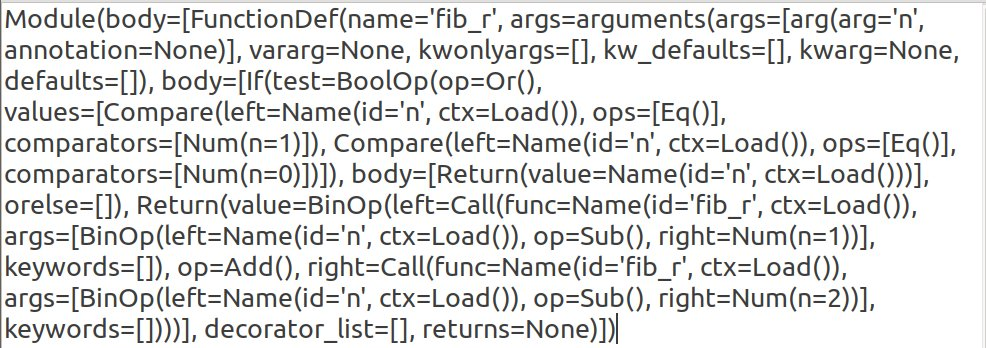
\includegraphics[width=\linewidth]{ast_fib_r}
  \caption{AST da função fib\_r(n) com ou sem comentário}
\end{figure}

Para corroborar que o cache funcionou, quando consultado o subdiretório "cache" do diretório ".intpy", verifica-se que não há adição de novos objetos serializados.

\subsection{Implementação e avaliação 4: possibilidade de análise a nível de bytecode para solucionar problemas de refatoração}
Da mesma forma que alterações de estilo e comentários podem invalidar o cache na implementação clássica de memoization, uma refatoração pode mudar o hash calculado. Neste caso, mesmo com a utilização de AST, o cache pode ser invalidado, uma vez que refatorações potencialmente vão gerar códigos com ASTs diferentes.

Isso foi confirmado implementando a alteração sugerida pelo comentário das análises anteriores, onde a expressão "n == 1 or n == 0" foi substituída pela expressão "n < 2", que no contexto do script apresentado tem a mesma semântica, ou seja, vai fornecer o mesmo resultado, mas tem uma sintaxe diferente, portanto gerará uma AST diferente.

\renewcommand{\lstlistingname}{Trecho de código}
\begin{lstlisting}[language=Python, caption=Alteração da expressão no código]
@deterministic
def fib_r(n):
    if n < 2:
        return n

    return fib_r(n-1) + fib_r(n-2)
\end{lstlisting}

O código anterior foi testado e mesmo com a implementação que compara o hash das ASTs, em relação a expressão anterior, o cache não foi recuperado conforme esperado. Este trabalho, apesar de confirmar o problema levantado, não conseguiu apresentar uma solução para o mesmo, mas procura identificar no teste a seguir um possível caminho de solução, através de análise e comparação a nível de bytecode, uma vez que os interpretadores fazem reduções a expressões equivalentes no nível de bytecode. Pode ser que este caminho tenha potencial para solucionar o problema.

\renewcommand{\lstlistingname}{Trecho de código}
\begin{lstlisting}[language=Python, caption=Comparação a nível de bytecode]
import inspect
import ast
import dis
import operator

def foo_1():
	a = 'Python'
	b = {'Python', 'Java'}
	print (a in b)

def foo_2():
	a = 'Python'
	b = {'Python', 'Java'}
	print (not a not in b)

def get_bytecode(source):
	ast_conv = ast.parse(source)
	bytecode = dis.Bytecode(compile(ast_conv, '<string>', 'exec')).dis()
	return bytecode

if __name__ == "__main__":
	source1 = inspect.getsource(foo_1)
	source2 = inspect.getsource(foo_2)
	bytecode1 = get_bytecode(source1)
	bytecode2 = get_bytecode(source2)
	print("Source 1")
	dis.dis(foo_1)
	print("Source 2")
	dis.dis(foo_2)
\end{lstlisting}

\renewcommand{\lstlistingname}{Trecho de código}
\begin{lstlisting}[language=bash, caption=Saída de comparação a nível de bytecode]
Source 1
7           0 LOAD_CONST               1 ('Python')
            2 STORE_FAST               0 (a)

8           4 LOAD_CONST               1 ('Python')
            6 LOAD_CONST               2 ('Java')
            8 BUILD_SET                2
           10 STORE_FAST               1 (b)

9          12 LOAD_GLOBAL              0 (print)
           14 LOAD_FAST                0 (a)
           16 LOAD_FAST                1 (b)
           18 COMPARE_OP               6 (in)
           20 CALL_FUNCTION            1
           22 POP_TOP
           24 LOAD_CONST               0 (None)
           26 RETURN_VALUE
Source 2
12          0 LOAD_CONST               1 ('Python')
            2 STORE_FAST               0 (a)

13          4 LOAD_CONST               1 ('Python')
            6 LOAD_CONST               2 ('Java')
            8 BUILD_SET                2
           10 STORE_FAST               1 (b)

14         12 LOAD_GLOBAL              0 (print)
           14 LOAD_FAST                0 (a)
           16 LOAD_FAST                1 (b)
           18 COMPARE_OP               6 (in)
           20 CALL_FUNCTION            1
           22 POP_TOP
           24 LOAD_CONST               0 (None)
           26 RETURN_VALUE
\end{lstlisting}

\subsection{Implementação e avaliação 5: análise de profiling das funções}
Outra análise que foi iniciada e que deve ser alvo de novas melhorias no IntPy é em relação a quais parte do código da infraestrutura são mais custosas computacionalmente. Isso faz com que a própria execução do IntPy concorra e some-se ao tempo de execução dos algoritmos gerais que estão sendo analisados. Esse comportamento é crítico principalmente para funções mais rápidas, mas, por outro lado, pode agregar uma característica importante ao IntPy, que com, tais aferições, poderia decidir se vale a pena ou não para um determinado caso, construir a infraestrutura do cache, uma vez que ela tem um custo que pode ser muitas vezes até maior que a própria execução principal. Incluir esta inteligência no IntPy parece ser uma vantagem muito interessante e uma análise de profiling pode ser o caminho para esta implementação.

Como prova de conceito para estudos iniciais, foi feita a análise de profiling de algumas execuções dos experimentos que foram executados através do módulo cProfile (\url{https://docs.python.org/3/library/profile.html}) do Python e foi verificado que para as primeiras execuções do cálculo de Fibonacci recursivo com memoization, que são mais custosas por causa da construção da infraestrutura do IntPy, para o Fib 35, aproximadamente 67\% do tempo de execução é gasto com as operações de "insert" e "commit" no banco de dados, mostrando ser um gargalo importante a ser solucionado.

Uma possível solução seria a execução de threads para efetuar estas operações, desassociadas do cálculo principal e retorno para o usuário do resultado.

\subsection{Implementação e avaliação 6: avaliando outros algoritmos - cálculo de potência}
Para complementar a análise, com o objetivo responder às questões de pesquisa, os testes de memoization com AST foram feitos para outros algoritmos, que realizam outros tipos de cálculos. Neste experimento é testado o cálculo de potência com implementação recursiva, para o caso de 100\textsuperscript{190}.

\renewcommand{\lstlistingname}{Trecho de código}
\begin{lstlisting}[language=Python, caption=Cálculo de potência: 100\textsuperscript{190}]
@deterministic
def pow(n, x):
    if x == 0 and True:
        return 1

    return n*pow(n, x-1)
    
if __name__ == "__main__":
    start = time.time()
    print(pow(100, 190))
    end = time.time()
    elapsed_time = end - start
    print(elapsed_time)
\end{lstlisting}

Na Tabela~\ref{tab:potrscache} e na Tabela~\ref{tab:potrccache} verificamos as execuções do cálculo de potência de 100 elev a 190 sem e com memoization, respectivamente. O cálculo implementado classicamente pode ser considerado rápido, se compararmos com nosso estudo de caso base, do cálculo de Fibonacci, portanto. O valor médio da execução sem cache foi de 0.0002 seg.

Já o valor com memoization foi de 2.20 seg na primeira execução, pois há a construção da infraestrutura do cache e o cálculo integral da potência e após isso mesmo as execuções mais rápidas (de 2 a 6), que utilizam o cache, não se mostram melhores que o código original. Na execução 6 foi feita a adição de comentário e o cache funcionou e na execução 7 foi feita uma alteração no código e o cache não funcionou, em ambos os casos, conforme esperado.
\begin{table}[H]
  \caption{Cálculo de potência recursivo sem memoization: 100\textsuperscript{190}}
  \label{tab:potrscache}
  \begin{tabular}{cl}
    \toprule
    Execução & Tempo de execução em seg\\
    \midrule
    1 & 0.0002491474151611328\\
    2 & 0.00014853477478027344\\
    3 & 0.00015211105346679688\\
    4 & 0.00025463104248046875\\
    5 & 0.00020885467529296875\\
  \bottomrule
\end{tabular}
\end{table}

\begin{table}[H]
  \caption{Cálculo de potência recursivo com memoization: 100\textsuperscript{190}}
  \label{tab:potrccache}
  \begin{tabular}{cl}
    \toprule
    Execução & Tempo de execução em seg\\
    \midrule
    1 & 2.2014591693878174\\
    2 & 0.005283355712890625\\
    3 & 0.004831552505493164\\
    4 & 0.00526738166809082\\
    5 & 0.005174875259399414\\
    6 & 0.005970001220703125\\
    7 & 1.998201608657837\\
  \bottomrule
\end{tabular}
\end{table}

\subsection{Implementação e avaliação 7: avaliando outros algoritmos - ordenação com quicksort}
Continuando as análises complementares, iremos implementar o algoritmo de ordenação quicksort, que é um algoritmo de ordenação muito eficiente. Será feito a mesma análise da avaliação anterior, com e sem memoization, com a seguinte sequência de números inteiros: [1, 3, 5, 2, 5, 0, 333, 2, 3, 10, 15, 20, 44, 33, 22, 64, 76, 87, 87, 98, 65, 100, 1234, 2, 345, 456, 343, 656, 767, 323, 4343, 6565, 6767, 8787, 9898, 98, 3434]

\renewcommand{\lstlistingname}{Trecho de código}
\begin{lstlisting}[language=Python, caption=Quicksort]
@deterministic
def quicksort(list):
    if len(list) <= 1 and True:
        return list

    pivot = list[0]
    equal = [x for x in list if x == pivot]
    greater = [x for x in list if x > pivot]
    lesser = [x for x in list if x < pivot]

    return quicksort(lesser) + equal + quicksort(greater)
    
if __name__ == "__main__":
    start = time.time()
    print(quicksort([1, 3, 5, 2, 5, 0, 333, 2, 3, 10, 15, 20, 44, 33, 22, 64, 76, 87, 87, 98, 65, 100, 1234, 2, 345, 456, 343, 656, 767, 323, 4343, 6565, 6767, 8787, 9898, 98, 3434]))
    end = time.time()
    elapsed_time = end - start
    print(elapsed_time)
\end{lstlisting}

Na Tabela~\ref{tab:quickrscache} e na Tabela~\ref{tab:quickrccache} verificamos as execuções do quicksort sem e com memoization, respectivamente. O cálculo implementado classicamente é mais rápido ainda que o exemplo anterior. O valor médio da execução sem cache foi da ordem entre 6 e 7 x10\textsuperscript{-5} seg.

Já o valor com memoization foi de 0.45 seg na primeira execução, pelas mesmas razões do exemplo anterior e após isso mesmo as execuções mais rápidas (de 2 a 6), que utilizam o cache, não se mostram melhores que o código original. Na execução 6 foi feita a adição de comentário e o cache funcionou e na execução 7 foi feita uma alteração no código e o cache não funcionou, em ambos os casos, conforme esperado.

\begin{table}[H]
  \caption{Quicksort recursivo sem memoization}
  \label{tab:quickrscache}
  \begin{tabular}{cl}
    \toprule
    Execução & Tempo de execução em seg\\
    \midrule
    1 & 7.462501525878906e-05\\
    2 & 6.818771362304688e-05\\
    3 & 6.818771362304688e-05\\
    4 & 6.699562072753906e-05\\
    5 & 7.033348083496094e-05\\
  \bottomrule
\end{tabular}
\end{table}

\begin{table}[H]
  \caption{Quicksort recursivo com memoization}
  \label{tab:quickrccache}
  \begin{tabular}{cl}
    \toprule
    Execução & Tempo de execução em seg\\
    \midrule
    1 & 0.45016908645629883\\
    2 & 0.006013631820678711\\
    3 & 0.005643367767333984\\
    4 & 0.005239009857177734\\
    5 & 0.005361795425415039\\
    6 & 0.005881071090698242\\
    7 & 0.44534778594970703\\
  \bottomrule
\end{tabular}
\end{table}

\subsection{Implementação e avaliação 8: avaliando outros algoritmos - cálculo de Fibonacci iterativo}
A última análise será feita novamente no algoritmo do cálculo de Fibonacci, mas para a implementação iterativa. É esperado que o algoritmo tenha um desempenho melhor que o recursivo, principalmente quando o número alvo vai aumentando, uma vez que a complexidade no tempo do algortimo iterativo é linear e a do algoritmo recursivo é exponencial, conforme pode ser visto na Figura 1. Em geral, algortimos recursivos são de mais fácil compreensão e reuso do que os iterativos, mas seu desempenho é inferior principalmente quando o números vão crescendo. Assim, é esperado que o algoritmo iterativo tenha o comportamento dos algoritmos mais rápidos, como os últimos que analisamos.

\begin{figure}[H]
  \centering
  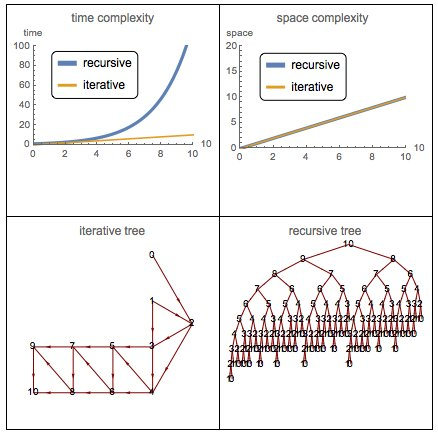
\includegraphics[width=\linewidth]{fib_10_rec_vs_it}
  \caption{Fibonacci de 10: recursivo vs iterativo. \newline Fonte: \url{www.demonstrations.wolfram.com}}
\end{figure}

\renewcommand{\lstlistingname}{Trecho de código}
\begin{lstlisting}[language=Python, caption=Sequência de Fibonacci iterativa com memoization]
def fib_it1(n):
	prev_prev = 0.0
	prev = 1

	for i in range(0, n-1):
		cur = prev_prev + prev
		prev_prev = prev
		prev = cur
	return cur

if __name__ == "__main__":   
    print(fib_it1(35))
    end = time.time()
    elapsed_time = end - start
    print(elapsed_time)
\end{lstlisting}

Na Tabela~\ref{tab:fibiscache} e na Tabela~\ref{tab:fibiccache} verificamos as execuções do Fibonacci iterativo sem e com memoization, respectivamente. O cálculo implementado classicamente é mais rápido ainda que o exemplo anterior. O valor médio da execução sem cache foi da ordem entre 6 e 7 x10\textsuperscript{-5} seg.

Já o valor com memoization foi de 0.45 seg na primeira execução, pelas mesmas razões do exemplo anterior e após isso mesmo as execuções mais rápidas (de 2 a 6), que utilizam o cache, não se mostram melhores que o código original. Na execução 6 foi feita a adição de comentário e o cache funcionou e na execução 7 foi feita uma alteração no código e o cache não funcionou, em ambos os casos, conforme esperado.

\begin{table}[H]
  \caption{Sequência de Fibonacci iterativa e sem memoization em Python}
  \label{tab:fibiscache}
  \begin{tabular}{crl}
    \toprule
    Execução & Resultado & Tempo de execução em seg\\
    \midrule
    1 & 9227465 & 1.239776611328125e-05\\
    2 & 9227465 & 8.344650268554688e-06\\
    3 & 9227465 & 8.106231689453125e-06\\
    4 & 9227465 & 9.059906005859375e-06\\
    5 & 9227465 & 8.58306884765625e-06\\
  \bottomrule
\end{tabular}
\end{table}

\begin{table}[H]
  \caption{Sequência de Fibonacci iterativa e com memoization em Python}
  \label{tab:fibiccache}
  \begin{tabular}{crl}
    \toprule
    Execução & Resultado & Tempo de execução em seg\\
    \midrule
    1 & 9227465 & 0.011674642562866211\\
    2 & 9227465 & 0.005118370056152344\\
    3 & 9227465 & 0.005065441131591797\\
    4 & 9227465 & 0.005356788635253906\\
    5 & 9227465 & 0.005749940872192383\\
    6 & 9227465 & 0.005084514617919922\\
    7 & 9227465 & 0.025156497955322266\\
  \bottomrule
\end{tabular}
\end{table}

\section{Trabalhos relacionados}
Entre os trabalhos descritos na literatura que tratam de memoization ou técnicas similares de cache para recomputação, no campo das linguagens de script o mais conhecido e reconhecido como implementação de referência é o IncPy \cite{guo2011using}(não confunda, é IncPy e não IntPy), que é uma implementação completa e automática de suporte à recomputação, fazendo análise dinâmica, rastreamento de dependência, persistência de cache, profiling e detecção de funções impuras. O problema prático é que para ser implementado o autor do trabalho programou milhares de linha de código em C para implementar um interpretador otimizado compatível com a versão 2.6.3 do Python, sendo assim ele só funciona com scripts escritos para esta versão. Após mais de 10 anos o interpretador não foi atualizado, o que inviabiliza sua utilização prática para vários experimentos. Mesmo assim, é o mais referenciado da área.

Além do IncPy, outros trabalhos foram desenvolvidos principalmente para Java, como o Cachetor\cite{nguyen2013cachetor}, MemoizeIt\cite{della2015performance} e Memcached\cite{fitzpatrick2004distributed}, utilizando uma ou mais das técnicas implementadas no IncPy mas com mais intervenção necessária. Cabe ressaltar que nenhum desses trabalhos consegue tratar o problema da evolução do software do ponto de vista de alteração de estilo, adição de comentários ou refatoração num ambiente de recomputação.

\section{Ameaças à validade}
Construção de infraestrutura sem solicitação de utilização do cache.

A utilização de forma indiscriminada do decorador pode degradar o desempenho.

Implementação limitada a programas escritos em Python.

Falta de testes aplicados a casos de uso reais.

\section{Trabalhos futuros}
Correção para não geração da infraestrutura de cache quando não utiliza o decorador.

Implementação da persistência em background (após retorno do resultado da execução).

Implementação para verificação de similaridade (testes, diff AST, bytecode).

Implementação de verificação do que vale a pena ou não utilizar a infraestrutura de cache (profiling, base, ML, fecho transitivo das chamadas, program slicing, etc).

Realização de testes com casos de uso reais.

Implementar técnica para classificar funções determinísticas e não-determinísticas.

\section{Conclusões}
Voltando às questões de pesquisa:
\begin{itemize}
\item \textbf{QP1:} {\textit{Como a adição de comentários, refatoração e alterações de estilo influenciam na velocidade da execução de scripts num cenário de recomputação? (H1: afirmação: a adição de comentários, refatoração e alterações de estilo influenciam)}}
\item \textbf{QP2:} {\textit{Que mudanças podem ser implementadas para reduzir esses efeitos e aumentar a abrangência da recomputação?}}
\item \textbf{QP3:} {\textit{Qual a aplicabilidade da recomputação diante de algoritmos de diferentes performances nativas?}}
\item \textbf{QP4:} {\textit{Qual a aplicabilidade da recomputação diante de algoritmos que podem ser implementados utilizando diferentes técnicas? (ex: implementação recursiva ou iterativa)}}
\end{itemize}

Há muito trabalho a ser feito.

Por outro lado, há muita oportunidade para crescimento da pesquisa neste tema (gargalos de velocidade em cenários diferentes, adição de novas técnicas, detecção de locais de aplicação, etc).

%%
%% The acknowledgments section is defined using the "acks" environment
%% (and NOT an unnumbered section). This ensures the proper
%% identification of the section in the article metadata, and the
%% consistent spelling of the heading.
\begin{acks}
To Robert, for the bagels and explaining CMYK and color spaces.
\end{acks}

%%
%% The next two lines define the bibliography style to be used, and
%% the bibliography file.
%%\bibliographystyle{ACM-Reference-Format}
\bibliographystyle{ieeetr}
\bibliography{art_cv2020_xrefs}

\end{document}
\endinput
%%
%% End of file 'art_cv2020_1short.tex'.